% \pagebreak[4]
% \hspace*{1cm}
% \pagebreak[4]
% \hspace*{1cm}
% \pagebreak[4]

\chapter{Background}
\ifpdf
    \graphicspath{{Design/DesignFigs/PNG/}{Design/DesignFigs/PDF/}{Design/DesignFigs/}}
\else
    \graphicspath{{Design/DesignFigs/EPS/}{Design/DesignFigs/}}
\fi

This chapter gives a brief overview of the features and classes of poetry that exist, along with why people are interested in writing them. We will discuss, critique and gather inspiration from the related work in the area of poetry generation that most relate to the approach taken in this paper. We then give brief overviews into the fields of Computational Linguistics and Computational Creativity, both of which are involved in the task of automatic poetry generation. These overviews are by no means complete or comprehensive, but should provide enough information for those not familiar with the areas to understand and appreciate this paper.

\section{Poetry Theory}

To fully comprehend the task that we are about to undertake, we need to have an understanding of poetry as an art form. It is ever-evolving and different styles have emerged over the years. Here we discuss those styles and the underlying reason for why poetry is written.

\subsection{The Purpose of Poetry}
\label{sec:purpose}
Merriam-Webster dictionary defines poetry as:\\
\emph{'writing that formulates a concentrated imaginative awareness of experience in language chosen and arranged to create a specific emotional response through meaning, sound, and rhythm.'}

Let us break this down:
\begin{itemize}
\item{\textit{\textbf{Formulates}} implies that there is method to the process of writing a poem.}
\item{\textit{\textbf{Concentrated}} accentuates the fact that poems are generally short, as they are counted in stanzas in lines rather than paragraphs and pages.}
\item{\textit{\textbf{Imaginative}} confirms the fact that this is a creative act, that has a level of non-determinism and need not be entirely realistic.}
\item{\textit{\textbf{Awareness of Experience}} embodies the need for general background knowledge based on a particular set of experiences that surface when writing a poem.}
\item{\textit{\textbf{Language Chosen and Arranged}} reiterates that this is a methodical and systematic art - words are chosen carefully with precise intention.}
\item{\textit{\textbf{Create a specific emotional response}} gives the main purpose of the poem - to express a feeling or an idea and elicit emotion in the reader.}
\item{\textit{\textbf{Through meaning, sound, and rhythm}} describes that this purpose is not reached purely by words, but other language features.}
\end{itemize}

To summarise, the purpose of poetry is to use one's imagination, knowledge and experience to trigger empathy about a particular subject matter. Poetry is a vehicle through which poets can share a very personal message that they want the reader to experience and remember. Poems are concise but have many layers of meaning that are subtle even to human readers and that only the best of poets can fully control. 

We must keep this in mind throughout the project, as it is important to realise that the features of poetry discussed in the next section are not arbitrary rules on form but purposeful techniques used to make the language more concise and effective.

\subsection{Features of Poetry}
\label{sec:features}

The earlier definition mentions the use of \textit{meaning, sound and rhythm} in poetry. These add an extra layer of subtext to poems to help the author remain concise while still getting the complete message across. We call these techniques \textit{features} of poetry throughout this paper. There are many features of poetry to address, but we have scoped this project down to concentrate on the following common ones.

\subsubsection{Rhyme}
\label{sec:rhyme}

\begin{figure}[h!]
\centering
\textit{
There once was a big brown \textbf{cat}\\
That liked to eat a lot of \textbf{mice}\\
He got all round and \textbf{fat}\\
Because they tasted so \textbf{nice}
}
\caption{A rhyming quatrain often used in teaching poetry}
\label{fig:rhyme}
\end{figure}
Two words rhyme when they sound similar when spoken out loud. \textit{Cat} and \textit{fat} in figure \ref{fig:rhyme} rhyme, as do \textit{mice} and \textit{nice}. Rhyming words need not be spelt similarly, for example, \textit{kite} and \textit{height}. 

Strict rhyme enforces the exact same sound while weak rhyme only requires that the vowel sounds are the same. Examples of weak rhyme are \textit{turtle} with \textit{purple} and \textit{tragedy} with \textit{strategy}. 

A piece of text has a rhyme scheme if there is a pattern of rhyme between its lines. For example, the poem in Figure \ref{fig:rhyme} has an \textit{ABAB} rhyme scheme.

Rhyme can also occur within a line (internal rhyme) or between words in the middle of different lines.

\textbf{Major Purposes} 
\begin{itemize}
\item{Pleasant to hear, making the listener feel more comfortable and listen carefully.} 
\item{As a mnemonic device.}
\item{Used at the end of lines of poetry and songs making the rhythmic structure more distinct.}
\end{itemize}


\subsubsection{Rhythm}
\label{sec:rhythm}
Rhythm is the pattern of emphasis of syllables that occurs in a line of poetry. There are three major ways of measuring rhythm, often used in tandem - syllabic, quantitative and accentual.

\begin{figure}[h!]
\centering
\textit{
The bartender said\\
to the neutron, 'For you, sir,\\
there will be no charge.'\\
}
\caption{A humourous Haiku}
\label{fig:haiku}
\end{figure}

\textbf{Syllabic rhythm} enforces a certain number of syllables to be used in a particular line of poetry. Haikus, for example, are three lines long with the first and last lines restricted to 5 syllables and the second to 7. An example is given in Figure \ref{fig:haiku}.

\textbf{Quantitative} measures use the fact that some syllables \textit{sound} longer than others when spoken out loud. Long sounding syllables are \textit{stressed} while short ones are \textit{unstressed}. 

\textbf{Accentual} measures are similar to Quantitative, but they work on the \textit{tendency to emphasize a particular syllable} when spoken out loud, rather than its length. It is important to note that a word's meaning can change depending on stress. For example, '\textbf{ob}ject' is a noun whereas 'ob\textbf{ject}' is a verb.

Lines of pre-defined patterns of stressed and unstressed syllables are called \textit{meters}. Lines with meter are made up of individual units called \textit{feet}. The five major foot types in poetry are given in Table \ref{tab:rhythm}.

\begin{table}[h!]
\centering
    \begin{tabular}{|l|l|l|}
    \hline
    Foot Type & Pattern                            & Example  \\ \hline
    iamb      & unstressed - stressed              & des\textbf{cribe} \\ \hline
    trochee   & stressed - unstressed              & \textbf{po}em     \\ \hline
    spondee   & stressed - stressed                & \textbf{popcorn}  \\ \hline
    anapest   & unstressed - unstressed - stressed & meta\textbf{phor} \\ \hline
    dactyl    & stressed - unstressed - unstressed & \textbf{po}etry   \\ \hline
    \end{tabular}
\caption{The major poetic foot types with their corresponding pattern and an illustrative example.}
\label{tab:rhythm}
\end{table}


The metre is formed by repeating feet, typically with up to six feet:
\begin{itemize}
\setlength{\itemsep}{0pt}
\item{Monometer: 1 foot}
\item{Dimeter: 2 feet}
\item{Trimeter: 3 feet}
\item{Tetrameter: 4 feet}
\item{Pentameter: 5 feet}
\item{Hexameter: 6 feet}
\end{itemize}

All Shakepeare's sonnets are written in iambic pentameter, i.e. five repetitions of unstressed-stressed syllables. The first line of his Sonnet II as an example:\\
\textit{When \textbf{for}ty \textbf{win}ters \textbf{shall} be\textbf{siege} thy \textbf{brow}}.

\textbf{Major Purposes}
\begin{itemize}
\item{Introduces a melody based on the natural intonations of speech.} 
\item{Adds a level of predictability and structure that resonates with readers and listeners.}
\item{Emphasizes the message by putting stress on the words that matter.}
\end{itemize}


\subsubsection{Sound Devices}
\label{sec:sound}
This project considers four types of sound devices.

The first is \textbf{onomatopoeia} - words that imitate or suggest sounds of particular sources. For example, the \textit{pow} of a punch or the \textit{tick-tock} of a clock. This technique has mostly been used in comic books to help the reader experience the sound of the scene to go with the image.

The next three devices are repetitions of a pattern of similar sounds. \textbf{Consonance} is the repetition of similar consonant sounds (e.g. \textit{pitter patter} repeats the 'p', 't', and 'r' sounds), while \textbf{assonance} is that of vowels (e.g. \textit{doom and gloom} repeats the 'oo' sound). \textbf{Alliteration} is a special case where the repeated sound occurs at the beginning of consecutive words. \textit{Zany zebras zigzagged through the zoo} has alliteration on the letter 'z'.

\textbf{Major Purposes}
\begin{itemize}
\item{Poets use onomatopoeia to help describe actions or atmosphere richly. A famous example is the nursery rhyme 'Old MacDonald', which uses onomatopoeia of the sounds that animals make to describe the farm, figuratively placing the reader or listener in the farm itself.} 
\item{Alliteration, consonance and assonance are pleasant to listen to when spoken out loud.}
\item{Can be used to add drama to an action.}
\item{Sometimes used to suggest danger.}
\end{itemize}


\subsubsection{Structure}
\label{sec:structure}
The structure of the poem is the organisation of its lines in a poem. The main unit is the \textit{stanza}, which is a fixed number of \textit{lines} grouped by rhythmical pattern.

There are four major types of stanza:
\begin{itemize}
\item{Couplet: 2 lines}
\item{Tercet: 3 lines}
\item{Quatrain: 4 lines}
\item{Cinquain: 5 lines}
\end{itemize}

Stanzas can also be called \textit{verses}, which have the added property of a rhyme scheme. A \textit{chorus} is a special type of verse that is repeated throughout a poem.

Features of the structure of a poem include:
\begin{itemize}
\item{The number of stanzas.}
\item{The number of lines per stanza.}
\item{The number and positions of repeated lines.}
\item{The number and positions of repeated stanzas.}
\item{Enjambment; the continuation of a sentence over a line-break}
\end{itemize} 

The Haiku in Figure \ref{fig:haiku} has a single tercet structure with no repetitions. Songs are generally several stanzas long, with a chorus interleaving longer non-repeating verses.

\textbf{Major Purposes}
\begin{itemize}
\item{Helps to guide the reader through the story.}
\item{Forces the poet to be more succinct and purposeful.}
\item{Manages the storyline - changes in stanza often suggest a change in perspective or message.}
\item{Repetition helps drive home the main message.}
\item{Ties several thoughts together into one continuous flow.}
\end{itemize} 

\subsubsection{Symbolism and Imagery}
\label{sec:symbol}
Symbolism and imagery are general terms for creating an overall image in the reader's mind by describing a subject or object as something else with desired qualities.

Techniques include:
\begin{itemize}
\item{\textbf{Metaphor}: an object is described as another object with a set of desirable characteristics. For example, saying someone is a lion immediately creates the image of bravery, intimidation and power.}
\item{\textbf{Simile}: an object or action is specifically described using an adjective or adverb, but compared to another object that is a stereotypical example of that description. The phrases 'like a' and 'as a' are often used, e.g. \textit{Runs like a cheetah}, \textit{Slippery as an eel}.}
\item{\textbf{Hyperbole}: unrealistic exaggeration, often used in tandem with metaphor e.g. \textit{Cried a river of tears}.}
\item{\textbf{Powerful Verb}: a more exciting way to describe an action using unusual verbs, e.g. \textit{Wormed through the crowd}.}
\item{\textbf{Personification}: using actions and properties associated with sentient objects to describe inanimate ones. Explained further in section \ref{sec:pragpers}}
\item{\textbf{Onomatopoeia}: as explained in section \ref{sec:sound}}, using imitations of known sounds to richly describe actions and atmosphere.
\end{itemize}

\textbf{Major Purposes}
\begin{itemize}
\item{Explain complex concepts concisely.}
\item{Induce empathy from the reader by relating it to something they understand.}
\end{itemize} 

\subsubsection{Context and Personification}
\label{sec:pragpers}
Poetry is similar to storytelling in that it has persona around whom the poem is written. Understanding who or what they are, their descriptions and their actions are all part of the underlying message that the poet wants to get across.

Personification is a technique used by poets to give inanimate objects life, expressing actions and descriptions as if it were sentient. This is a powerful technique that relates to imagery, helping poets make abstract messages clearer. For example, \textit{the moon smiled} gives the moon life by describing it as having performed a sentient action with full intention of doing so. Noting the use of personification can make the context of the poem clearer, as inanimate objects are often the subject of the poem.

\textbf{Major Purposes}\\
Context is the underlying message in its bare form. It is the story that the poet wishes to tell and guides the use of all other features.

In this paper, we aim to extract characters and differentiate them by their descriptions and actions. This is vital in understanding the poem and can help us generalise the uses of features when attempting to produce a coherent story as the backbone to the generated poem. Furthermore, it will help determine the type of poem (narrative, lyrical, descriptive etc.) and will help guide generation of poems of a particular type. 


\subsection{Classification of Poetry}

We define a type of poetry as a particular form of poem with a set of unique features, including those described in the previous section. Some types are very popular and have had their styles, features and purposes documented and taught. Out of these grew categories of different types that tend to be used for similar purposes.

This project attempts to derive these categories and some popular types of poetry by analysing many comparable poems.

\subsubsection{Categories}

There are many types of poem all with different form. However, there are only three main categories of purpose for a poem:

\begin{enumerate}
\item{\textit{Lyrical} poems have an identifiable speaker whose thoughts and emotions are being expressed in the poem. This means that poems of this category have very few characters, a song-like structure and tend to be in a reflective tone, generally using a lot of symbolism. Maya Angelou's \textit{I Know Why The Caged Bird Sings} is an example of this, along with many songs.}
\item{\textit{Descriptive} poems describe the surroundings of the speaker. This is identifiable by the use of adjectives and complex imagery. Many objects may appear in this type of poem to be able to give an in-depth description of the environment and atmosphere. There will be very few action verbs used.}
\item{\textit{Narrative} poems concentrate on telling a story. It therefore has a coherent plot line, several characters with explicit relationships between them, action and climax. Ballads and Epics are types of narrative poems.}
\end{enumerate}

Some popular poem types do not fall under any one bracket as they can be used in any of the above categories. Examples include Haikus and Limericks.

\subsubsection{Popular Types}
As well as determining the category of poems, we aim to be able to detect and reproduce some popular types of poetry. For this project, we will concentrate on:
\begin{itemize}
\item{\textit{Haiku:} single tercet structure with 5-7-5 syllabic rhythm.}
\item{\textit{Limerick:} single cinquain structure with AABBA rhyme scheme. Lines 1, 2 and 5 have 7-10 syllables, while lines 3 and 4 have 5-7 syllables. The first line tends to begin with "There was a..." and ending with a person or location. Limericks are usually used for humour as the last line is generally a punchline.}
\item{\textit{Sonnet:} 14 lines, each in iambic pentameter with an ABAB CDCD EFEF GG rhyme scheme, i.e. three quatrains followed by a rhyming couplet.}
\item{\textit{Elegy:} usually used to mourn the dead, its lines alternates between dactylic hexameter and pentameter in rhythm. It has no particular rhyme scheme, although does still use rhyme. }
\item{\textit{Ode:} Description of a particular person or thing, using plenty of similes, metaphors and hyperbole.}
\item{\textit{Ballad:} Tells a story and has a number of quatrains, each with an AABB rhyme scheme. Lines alternate between iambic tetrameter and iambic trimeter.}
\item{\textit{Cinquain:} as the name suggests, this has 5 lines. They are not rhymed, but have a 2-4-6-8-2 syllabic pattern. }
\item{\textit{Riddle:} Riddles describe things without telling what it is, using anaphora to refer to it. Ususally told in a number of rhyming couplets.}
\item{\textit{Free Verse:} No particular features attached to this type.}
\end{itemize} 


\section{Lessons from Related Work}
\label{sec:related_work}
This section looks at six important previous attempts at automatic poetry generation. They each have some aspect of investigation or experimentation that have influenced this project. Conversely, each of these attempts has its limitations that we look to overcome in this project.

\subsection{Actively Gather Inspiration}

Colton et al. published a paper in the International Conference of Computational Creativity 2012\cite{colton2012full}, whose main objective was to describe the first poetry generation system that satisfied the FACE Descriptive model\cite{colton2011computational}. It is a \textit{Form Aware}\cite{manurung2004evolutionary} implementation that constructs templates of poems based on constraints of poetic features. 

\begin{figure}[h!]
\begin{multicols}{2}
It was generally a bad news day. I read an article in
the Guardian entitled: “Police investigate alleged race
hate crime in Rochdale”. Apparently, “Stringer-Prince,
17, has undergone surgery following the attack on
Saturday in which his skull, eye sockets and
cheekbone were fractured” and “This was a
completely unprovoked and relentless attack that has
left both victims shocked by their ordeal”. I decided to
focus on mood and lyricism, with an emphasis on
syllables and matching line lengths, with very
occasional rhyming. I like how words like attack and
snake sound together. \columnbreak
I wrote this poem.\\
\textit{Relentless attack\\
a glacier-relentless attack\\
the wild unprovoked attack of a snake\\
the wild relentless attack of a snake\\
a relentless attack, like a glacier\\
the high-level function of eye sockets\\
a relentless attack, like a machine\\
the low-level role of eye sockets\\
a relentless attack, like the tick of a machine\\
the high-level role of eye sockets\\
a relentless attack, like a bloodhound
}
\end{multicols}
\caption{The Guardian article used for inspiration(left) and the resulting poem(right).}
\label{fig:face}
\end{figure}

The most interesting point of this paper was its admission that inspiration cannot come from the technology and must come from the user. By taking this into account, it now takes inspiration from news articles as seen in Figure \ref{fig:face}. However, since its objective was focused on passing a particular evaluation model, the poems created by this system are relatively simple and the processes rudimentary - using randomness rather than semantic applicability in word selection.

\subsection{Constrain to Improve Creativity}
\label{sec:con}
Recently, Toivanen et al. attempted a solution that used off-the-shelf constraint solvers\cite{toivanen2013harnessing} to produce poetry. Their solution, illustrated in figure \ref{fig:con1}, also received inspiration from external sources. This is used to build the set of candidate words, form requirements and content requirements that are passed into a constraint solver with a manually encoded static constraint library powered by Answer Set Programming.

\begin{figure}[h!]
\centering
\includegraphics[width=140mm]{Constraint}
\caption{Complete poetry composition workflow.}
\label{fig:con1}
\end{figure}

\begin{figure}[h!]
\begin{multicols}{2}
N SG VB, N SG VB, N SG VB!\\
PR PS ADJ N PL ADJ PRE PR PS N SG:\\
– C ADV, ADV ADV DT N SG PR VB!\\
\columnbreak DT N SG PRE DT N PL PRE N SG!\\
\textit{Music swells, accent practises, theatre hears!\\
Her delighted epiphanies bent in her universe:\\
– And then, singing directly a universe she disappears!\\
An anthem in the judgements after verse!
}
\end{multicols}
\caption{The POS template used for constraint input(left) and the resulting poem(right).}
\label{fig:con2}
\end{figure}

The idea that constraints do not hinder but rather help the creative process is an attractive one for Computational Creativity research. Constraining words and other requirements for each particular word position is a natural technique for constraint programming, but extremely restrictive. First, the size of each line must be defined by number of words \textit{and then} by rhythm and other poetic features. Secondly, once the candidate words are chosen there is no scope for further filtering. Finally, the structure of the poem in terms of its parts-of-speech (section \ref{sec:syntax}) tags must be defined beforehand and is taken from previous poems of the same type, as seen in Figure \ref{fig:con2}. Even though this is an efficient method that has produced impressive results, it is too restricted to produce truly creative work.

\subsection{Learn from Experience}
\label{sec:RKCP}

Ray Kurtzweil Cybernetic Poet (RKCP), created by Kurtzweil himself\cite{kurzweil1999ray}, addresses the issue of having a predefined template. He uses a stochastic approach that utilises of n-grams to build lines from words. The system was trained on a selection of poems that created a template and n-gram corpus from those poems. RKCP would use this to create similar types of poems. Some heuristics were employed to ensure that poems were not exact copies of other poems and to maintain a coherent theme.

\begin{figure}[h!]
\centering
\textit{
Scattered sandals\\
a call back to myself,\\
so hollow I would echo.
}
\caption{A haiku written by Ray Kurzweil's Cybernetic Poet after reading poems by Kimberly McLauchlin and Ray Kurzweil}
\label{fig:rkcp}
\end{figure}

This method is more flexible and has granular word selection. However, the vocabulary would still be limited and the form of the poem is not well defined due to being probabilistic. We can see that in Figure \ref{fig:rkcp}, the attempted Haiku has a syllabic rhythm is 4-6-7 as opposed to the required 5-7-5. A specific purpose or storyline is not definable and the use of imagery is only probabilistic. A lot also depends on the poems in the corpus, limiting semantic capabilities and word selection quality.


\subsection{Choose Words Carefully}
\label{sec:mcg}
MCGONAGALL\cite{manurung2004evolutionary} takes a semantic representation of a sentence, called \textit{semantic expressions}, as input into an NLG system. For example, the semantic expression of \textit{"John loves Mary"} would be \textit{\{john(j), mary(m), love(l, j, m)\}}

These are used as starting points for initialisation of his evolutionary system that uses stochastic methods to determine the best values to be carried forward to further iterations.

\begin{figure}[h!]
\centering
\textit{
They play. An expense is a waist.\\
A lion, he dwells in a dish.\\
He dwells in a skin.\\
A sensitive child,\\
he dwells in a child with a fish.\\
}
\caption{Resulting MCGONNAGAL poem when seeded with a couple of lines of Hilaire Belloc.}
\label{fig:mcg}
\end{figure}

\begin{figure}[h!]
\centering
\includegraphics[width=100mm]{lion}
\caption{Semantically enriched lexical entry for \textit{lion} in MCGONNAGAL}
\label{fig:lion}
\end{figure}

Of particular note is the structure of a lexical entry into the system. It is enriched with much semantic information, as in Figure \ref{fig:lion}, that backs up the fitness score and helps MCGONAGALL form syntactically and semantically correct sentences. We will use much of his ideas in this area. However, contextual coherence is lacking because of the restrictions imposed on evolution. It does not take particular types of poetry into account and there is little scope for creativity due to the strictness of grammar generated. 


\subsection{Derive Insight from Worldly Knowledge}
Tony Veale's daring approach to knowledge-based poetry generation\cite{veale2013less} concentrates on symbolism and imagery - arguably the hardest tasks in automatic poetry generation. He uses norms and stereotypes to build a structure that uses various words to describe objects and derive stereotypical characteristics. Out of this grew a very useful tool - Metaphor Magnet\cite{vealespecifying}, which was used to create the impressive poetry shown in Figure \ref{fig:veale}.

\begin{figure}[h!]
\centering
\textit{
My marriage is an emotional prison\\
Barred visitors do marriages allow\\
The most unitary collective scarcely organizes so much\\
Intimidate me with the official regulation of your prison\\
Let your sexual degradation charm me\\
Did ever an offender go to a more oppressive prison?\\
You confine me as securely as any locked prison cell\\
Does any prison punish more harshly than this marriage?\\
You punish me with your harsh security\\
The most isolated prisons inflict the most difficult hardships\\
O Marriage, you disgust me with your undesirable security\\
}
\caption{'The legalized regime of this marriage', a poetic view of marriage as a prison}
\label{fig:veale}
\end{figure}

His methods have obvious limitations in that they do not consider rhyme, rhythm or any other poetic feature other than symbolism. However, we will take advantage inspiration from the idea of using norms and stereotypes to give this system more symbolic choices of words and phrases.

\subsection{Dare to be Different}
WASP is one of the first attempts at an automatic poetry generator. It is a rule based system that takes a set of words, a set of verse patterns and returns a set of verses\cite{gervas2000wasp}. It uses heuristics to guide the construction to fit structure, but no semantic limitations are enforced.

This has obvious limitations but Gervas, the creator of this system, does make a good point that poetry's creativeness is somewhat down to daringness of transgression. We keep this in mind to allow some level of randomness and mutation from expected norms in this project. 

%https://www.era.lib.ed.ac.uk/bitstream/1842/314/1/IP040022.pdf
%All in docs
%http://link.springer.com/chapter/10.1007/3-540-46119-1_7#page-1
%http://citeseerx.ist.psu.edu/viewdoc/download?doi=10.1.1.126.1464&rep=rep1&type=pdf
%http://delivery.acm.org/10.1145/1880000/1870709/p524-greene.pdf?ip=82.31.135.169&id=1870709&acc=OPEN&key=BF13D071DEA4D3F3B0AA4BA89B4BCA5B&CFID=397642531&CFTOKEN=69509660&__acm__=1390863256_1cb8f68563ec050ead2a0b910996fc19

\section{Brief Overview of Computational Creativity}
Simon Colton and Geraint Wiggins define research in this area as: \\
\textit{The philosophy, science and engineering of computational systems which, by taking on particular responsibilities, exhibit behaviours that unbiased observers would deem to be creative.}\cite{colton2012computational}

In the context of automatic poetry generation, we are creating a system that \textit{takes on the responsibility} of generating aesthetically pleasing, meaningful and novel poems. The poems still need to be sufficiently similar to existing works created by humans such that it \textit{exhibits behaviour} to which \textit{unbiased observers} can relate and recognise.

This definition has evolved from one where behaviour was \textit{deemed creative if and only if it can be exhibited by humans}\cite{wiggins2006searching}. However, recent developments in the area have lead to the requirement of more quantitative measures for evaluation than Turing-style tests, such as the FACE and IDEA descriptive models\cite{colton2011computational}.

This area of research has come under scrutiny for philosophical reasons, but has had support from Alan Turing and other pioneers of Artificial Intelligence. It has since been accepted as a valid area of research, with the annual International Conference on Computational Creativity heading into its fifth year.

Successes of Computational Creativity:
\begin{itemize}
\item{Simon Colton's \textit{Painting Fool}\cite{colton2012painting} produced paintings that managed to trick art lovers into believing that it was the work of a talented human artist. An example is given in Figure \ref{fig:chair}.}
\item{\textit{JAPE}\cite{binsted1997computational}, created by Ritchie and Binsted in 1994 was given a general, non-humorous lexicon and generated puns as answers to questions. For example:\\\textit{Q:What do you call a strange market?\\ A: A bizarre bazaar}.}
\item{\textit{Iamus} by Gustavo Diaz-Jerez\cite{diaz2011composing}, which composed music entirely on its own that was then recorded by London Symphony Orchestra.}
\item{\textit{The Policeman's Beard is Half Constructed}\cite{chamberlain1984policeman} is recognised for being the first book, which included some poetry, to have been written entirely by a computer program, RACTER.}
\end{itemize} 

\begin{figure}[h!]
\centering
\includegraphics[width=100mm]{Chair}
\caption{Chair \#17 at the Performing Sciences Exhibition, La Maison Rouge, Paris, Sept 2011}
\label{fig:chair}
\end{figure}
%https://www.cs.helsinki.fi/webfm_send/571
%http://computationalcreativity.net/iccc2014/wp-content/uploads/2013/09/ComputationalCreativity.pdf

\subsubsection{Semantic Networks of Common Sense}
\label{sec:common-sense-bg}

Tom De Smedt uses the idea that the mind can be modelled as a search space of \textit{concepts} and relations between them. to model creativity\cite{creativitynetwork}. He proposes a network with concepts at the nodes and relations between them, perhaps of a specific type, are the edges.

In our case, these concepts are represented by words or phrases that have literal and symbolic meaning. The number of concepts in the space and how words relate to each other are determined by knowledge and experience.

If we think of a \textit{cat} as a concept, it would be directly related to other concepts such as \textit{dog} and \textit{mouse}. These are \textit{mundane} associations between concepts.

Concepts are defined in this network by looking at the outgoing neighbours of its node. This is called the concept \textit{halo}. Conversely, the \textit{field} of a concept acts as a classification by finding all neighbours that relate to it, rather than from it. A subgraph of the halo and field of the concepts \textit{cat} and \textit{feed.v} respectfully are shown in Figure \ref{fig:concept-halo-field}.

\begin{figure}[H]
\centering
\begin{subfigure}[t]{0.9\textwidth}
	\centering
    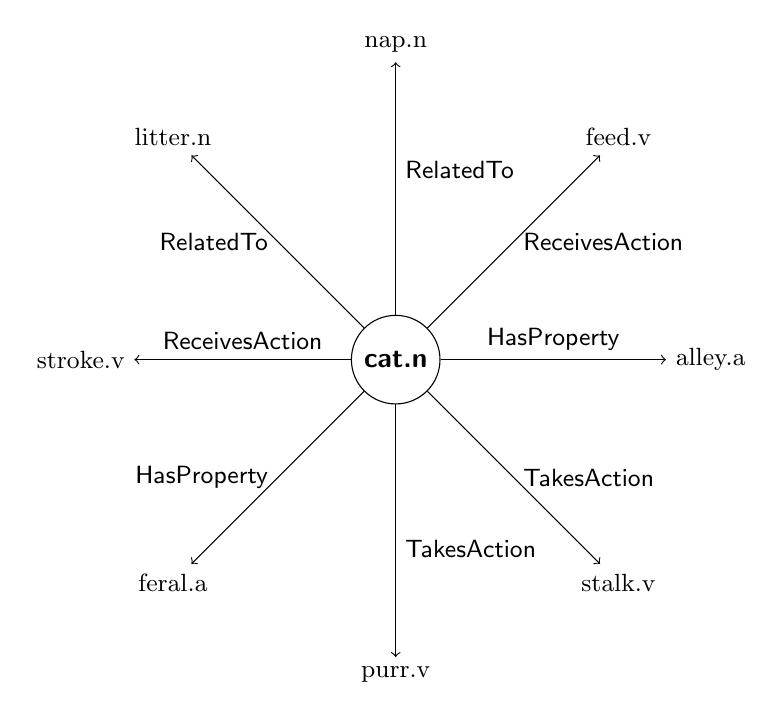
\begin{tikzpicture}[->, node distance=4cm,main node/.style={circle, draw, font=\sffamily\bfseries}]
        \tikzstyle{every node}=[font=\small]
        
          \node[main node] (1) [] {cat.n};
          \node[] (3) [above of=1]{nap.n};
          \node[] (4) [right of=1] {alley.a};
          \node[] (5) [below of=1] {purr.v};
          \node[] (6) [left of=1] {stroke.v};
          \node[] (7) [above right of=1] {feed.v};
          \node[] (8) [below right of=1] {stalk.v};
          \node[] (9) [below left of=1] {feral.a};
          \node[] (10) [above left of=1] {litter.n};

          \path[every node/.style={font=\sffamily\small}]
            (1) edge node [above right] {RelatedTo} (3)
               	edge node [above] {HasProperty} (4)
               	edge node [below right] {TakesAction} (5)
               	edge node [above] {ReceivesAction} (6)
                edge node [right] {ReceivesAction} (7)
                edge node [right] {TakesAction} (8)
                edge node [left] {HasProperty} (9)
                edge node [left] {RelatedTo} (10);
              
        \end{tikzpicture}
    \caption{Concept halo for \textit{'cat.n'}}
\end{subfigure}
\begin{subfigure}[t]{0.9\textwidth}
	\centering
   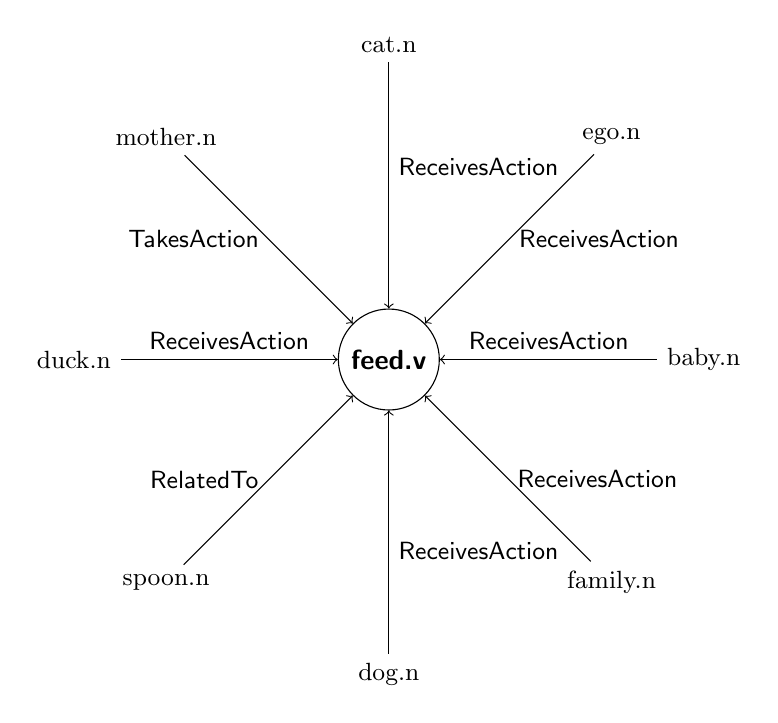
\begin{tikzpicture}[<-, node distance=4cm,main node/.style={circle, draw, font=\sffamily\bfseries}]
           \tikzstyle{every node}=[font=\small]
           
             \node[main node] (1) [] {feed.v};
             \node[] (3) [above of=1]{cat.n};
             \node[] (4) [right of=1] {baby.n};
             \node[] (5) [below of=1] {dog.n};
             \node[] (6) [left of=1] {duck.n};
             \node[] (7) [above right of=1] {ego.n};
             \node[] (8) [below right of=1] {family.n};
             \node[] (9) [below left of=1] {spoon.n};
             \node[] (10) [above left of=1] {mother.n};
   
             \path[every node/.style={font=\sffamily\small}]
               (1) edge node [above right] {ReceivesAction} (3)
                  	edge node [above] {ReceivesAction} (4)
                  	edge node [below right] {ReceivesAction} (5)
                  	edge node [above] {ReceivesAction} (6)
                   edge node [right] {ReceivesAction} (7)
                   edge node [right] {ReceivesAction} (8)
                   edge node [left] {RelatedTo} (9)
                   edge node [left] {TakesAction} (10);
                 
           \end{tikzpicture}
    \caption{Concept field for \textit{'feed.v'}}
\end{subfigure}
\caption{Example concept halo and field}
\label{fig:concept-halo-field}
\end{figure}

If we were to look at \textit{paths} in the network, we can realise relationships between concepts that are less mundane, and therefore more creative.

For example, we may travel along the path \textit{cat $\rightarrow$ meow $\rightarrow$ loud $\rightarrow$ fire alarm} to create an analogy between the cats and fire alarms.

Since this knowledge is modelled as a graph, we are able to use standard graph algorithms such as Dijkstra's shortest path\cite{dijkstra1959note} to find similarity between concepts.

\paragraph{ConceptNet}
\label{sec:conceptnet}
ConceptNet\cite{liu2004conceptnet} is an attempt to build a single source of \textit{'things computers should know about the world'} using the idea of a semantic network of concepts.

It gathers its knowledge from an array of sources but large amounts come from Wikipedia. Edges represent \textit{relations} between concepts and come in various types including:

It also provides functional interfaces such as finding the closest concept to a given number of concepts and similarity between concepts.

\section{Brief Overview of Computational Linguistics}
Computational Linguistics is a wide area of research, covering Speech Recognition, Natural Language Processing and Generation and with overlaps in several other areas such as Machine Learning and Knowledge Representation. In fact, Daniel Jurafsky and James H. Martin needed almost a thousand pages to cover the foundations of this area\cite{jurafsky2000speech}.

Automatic poetry generation borrows many techniques and terminology from Computational Linguistics. Here we will briefly discuss the major ones in general and in the context of machine poetry analysis and generation. For an in depth general study of Computational Linguistics, we refer the interested reader to Jurafsky and Martin's book.
%http://www.cse.iitk.ac.in/users/mohit/Speech-and-Language-Processing.pdf

\subsection{Words}
\label{sec:words}
Words are the fundamental building blocks of language. They have been studied for the creation of spell-checkers, text-to-speech synthesis and automatic speech recognition. Two major subsets where poetry is concerned is the study of pronunciation and morphology. 

The CMU Pronunciation Dictionary\cite{weide1998cmu} has taken steps towards computationally modelling the phonetics of words, using the ARPAbet phoneme set (see Table \ref{tab:arpa} in the Appendix). It is highly important for poetry generation as it helps machines reason about rhyme and sound devices by simply comparing phonemes. It has over 133,000 words mapped to corresponding pronunciations.

To illustrate how this works, let us take two words that are spelled differently but pronounced the same - \textit{kite} and \textit{height}. The Jaro-Winkler distance, a normalised score of similarity between strings, for the tail of these words (in search of rhyme) gives 51.11\%, indicating that it is barely probable that they rhyme if we only looked at spelling. Their corresponding phoneme sets are \textit{'K AY1 T'} and \textit{'HH AY1 T} respectively. Now it is trivial to compare them computationally and see that the tails are exactly the same and the words therefore rhyme.

Notice the '1' appended to the 'AY' phonemes. Vowel phonemes come with a digit appended to them that defines the emphasis placed on this syllable:
\begin{itemize}
\item{0: unstressed}
\item{1: stressed}
\item{2: light/secondary stress}
\end{itemize}

Morphology of words is the study of putting words together with \textit{morphemes}, the smallest unit of grammar. To use Jarufsky and Martin's example, the word \textit{fox} consists of a single morpheme that is itself, but \textit{cats} has two morphemes, \textit{cat} and \textit{-s}. This is of vital importance in our project as we need to understand the difference between different forms of the same word and how they relate to context. Furthermore, when generating text we wish to produce coherent grammar with consistent tense and perspective.

The CLiPS Pattern library has a number of tools for morphology of words. It provides a method of changing a word into its first, second or third person version, pluralisation and finding superlatives.\cite{de2012pattern}

%http://delivery.acm.org/10.1145/980000/972475/p313-marcus.pdf?ip=82.31.135.169&id=972475&acc=OPEN&key=BF13D071DEA4D3F3B0AA4BA89B4BCA5B&CFID=397642531&CFTOKEN=69509660&__acm__=1390858444_560bb7766479576772371b53b664bc15

\subsection{Syntax}
\label{sec:syntax}
Syntax is the glue that binds words together. It gives us an understanding of the grammatical relationship between words and guides the building of phrases and sentences.

\subsubsection{The Penn Treebank Tagset}

Core to this area of research is \textit{part-of-speech (POS)} analysis, which provides a model for grouping words together correctly, taking into account how words depend on each other. The big success story in this area is The Penn Treebank Tagset, an enormous corpus of annotated POS information \cite{marcus1993building}. The full tagset is given in Table \ref{tab:penn} in the Appendix. This accelerated progress of research in the area, as the paper had expected. 

From these POS tags, we are able to create \textit{grammars}, the structural rules of phrases and sentences, and \textit{parsers} for those grammars that are able to extract grammatical structure from unstructured text.

For example, the phrase \textit{John loves Mary} would be represented as in Figure \ref{fig:parse} if parsed with a grammar based on The Penn Treebank tagset.

\begin{figure}[h!]
\centering
\includegraphics[width=60mm]{Treebank}
\caption{Parse tree of \textit{'John loves Mary'}}
\label{fig:parse}
\end{figure}

Python's Natural Language Toolkit (NLTK)\cite{bird2009natural} is a suite of text processing libraries, corpora and lexical resources that is heavily used in this project, particularly for syntactical purposes. It will allow us to use The Penn Treebank tags as well as produce our own grammar and parser that can be used to parse most poetry. This is a challenge because we cannot expect poetry to follow grammatical rules as strictly as discourse. However, the pay-off will be that we can model the context of the poem, leading to better analysis of semantics and pragmatics of poetry.
%http://www.postgradolinguistica.ucv.cl/dev/documentos/49,578,Noam%20Chomsky%20-%20Syntactic%20Structure.pdf

\subsubsection{Stanford Dependencies}
\label{sec:stanford-deps}
The Stanford Dependencies\cite{de2008stanford} is another representation based around the relationships between words. All dependency relations are strictly binary and come in various types depending on the participants, called the \textit{governor} and the \textit{dependent}.

It aims to make extraction of textual relationships more approachable to those without linguistic expertise by using more colloquial relationships, such as subjects and objects of a sentence. We represent the dependencies of a sentence as directed graphs with words at the nodes and the dependency relations as the edges between them. Figure \ref{fig:shopkeeper-deps} shows this for the sentence \textit{'The shopkeeper told the customer to have a nice day'}

\begin{figure}[h!]
\centering
\includegraphics[width=140mm]{shopkeeper-deps}
\caption{TurboParser Semantic Dependency parse for the shopkeeper example.}
\label{fig:shopkeeper-deps}
\end{figure}

This was parsed using TurboParser\cite{turboparser}.


\subsection{Semantics}
\label{sec:semantics}
Noam Chomsky used the famous example \textit{'Colourless green ideas sleep furiously'} to show that a valid grammatical syntax can be completely nonsensical\cite{chomsky2002syntactic}. This illustrates the importance of the study of semantics; the meaning of words and phrases, as well as pragmatics; the way context affects semantics. Suppose the context around Chomsky's example was a person with old (black-and-white, colourless) ideas of making money (green) that he wants to bring back (was put to sleep, but not peacefully), then this line would make some sense in a poetic way.

We first introduce the concepts of \textit{anaphora} and \textit{presuppostions} and techniques for resolving them. We then move on to discussing two current methods of understanding semantics in natural language; Discourse Representation Theory and Semantic Role Labelling.

\subsubsection{Anaphora Resolution and Presupposition Projection}
\label{sec:arback}
In linguistics, \textit{anaphora} is the technique of using words that are used to refer to another object within a specific context. For example, the sentences \textit{'Joe put on a coat because he felt cold'} and \textit{'Because he felt cold, Joe put on a coat'} are both anaphoric, with \textit{'he'} being the anaphor that refers to 'Joe', who in the earlier sentence is referred to as the \textit{antecedent} and in the latter as the \textit{postcedent} because of the relative ordering of the word and its anaphor.

Presupposition is a similar technique, except that it works on implicit assumptions about the context. For example, the sentence \textit{'The cat chased the mouse, but it managed to evade the feline.'} uses the assumption that the cat is a feline. It then projects this as a presupposition to avoid re-using the same word or introducing anaphora, while still indicating to the same object. This is a very useful linguistic technique, especially when used to make temporal inferences. The sentence \textit{'Joe stopped playing the piano'} has the implicit assumption that Joe once played the piano.

Resolving anaphora and presupposition in text is an ongoing research area in Computational Linguistics. Various tools have been developed using a variety of techniques that are not discussed here. It is worth noting, though, that existing solutions generally do not use domain-specific or linguistic knowledge.

\subsubsection{Discourse Representation Theory}
\label{sec:drt}
Discourse Representation Theory (DRT)\cite{kamp1993discourse} is a framework for investigating semantics of natural language proposed by Hans Kamp. Abstract mental representations of DRT are Discourse Representation Structures (DRSs), which are designed to combine meaning across sentences and cope with anaphora (e.g. using pronouns in place of nouns, see Section \ref{sec:arback}). 

Using Kamp's example, if we take the sentence \textit{A farmer owns a donkey} and convert it into a DRS, we get the following notation:\\
\texttt{\{[x,y: farmer(x), donkey(y), own(x,y)]\}}

If we then say \textit{He beats it.}, it will produce:\\
\texttt{\{[x,y,z,w: farmer(x), donkey(y), own(x,y), PRO(z), PRO(w), beat(z,w)]\}}

We can then use anaphora resolution on this DRS to produce:\\
\texttt{\{[x,y: farmer(x), donkey(y), own(x,y), beat(x,y)]\}}

We can see that this is similar to the notation used by Manurung in MCGONNAGAL, described in section \ref{sec:mcg}.

This method has evolved over the years to take tense and aspect into account, providing temporal reasoning in natural language sentences. Accuracy of anaphora and presupposition (e.g. saying 'animal' instead of 'cat', see Section \ref{sec:arback}) resolution has improved with the use of the third-party tools in combination with the ideas of Blackburn and Bos\cite{blackburn2008computational}.

Extending this example, we may wish to model the sentence \textit{Every farmer who owns a donkey beats it.}. DRT provides an elegant solution for this using first order logic style 'for all':\\
\texttt{\{[x][y][farmer(x), donkey(y), own(x,y) $\rightarrow$ beat(x,y)]\}}

This allows us to provide background knowledge to the system and make inferences on it. As a result of its usefulness in many applications, NLTK has included DRS manipulation and anaphora resolution into its core semantics package.

Johan Bos and his team have begun the Groningen Meaning Bank (GMB) project\cite{BasileBosEvangVenhuizen2012LREC}, a large semantically annotated corpus in lieu of The Penn Treebank, in the attempt to bring the same success and acceleration to this sub-field of research. They use DRT as the backbone to an assembly of third-party tools to annotate semantics, as can be seen in Figure \ref{fig:gmb}. However, the GMB project is still in early stages and has only annotated open license news articles up until now, which is not a suitable corpus for many use-cases, including poetry generation.

\begin{figure}[h!]
\centering
\includegraphics[width=125mm]{Groningen}
\caption{Semantic structure of the sentence \textit{Smoking causes diseases.}}
\label{fig:gmb}
\end{figure}
%http://www.let.rug.nl/bos/pubs/BasileBosEvangVenhuizen2012LREC.pdf
%http://aclweb.org/anthology/W/W11/W11-2819.pdf
%http://www.let.rug.nl/bos/pubs/BasileBosEvangVenhuizen2012LREC.pdf

DRT in general is very effective when dealing with rule-based knowledge bases, in lieu of declarative logic programming. Its proficiency at anaphora and presupposition resolution and handling "donkey phrases" make it applicable to question-answer systems, where usefulness comes in determining truth or falsity of sentences.

However, it may not be an effective model for semantic relations that require classification of different types of phrases and the roles of words in a sentence. It also requires a very comprehensive and flexible grammar to be able to convert a large variety of English sentences into Discourse Representation Structures, especially if the sentences may not have perfect grammar as in poetry. For this, we use a method called Semantic Role Labelling.

\subsubsection{Semantic Role Labelling}
Semantic Role Labelling (SRL) is best described with an example. Take the sentence:
{\centering\textit{"The shopkeeper told the customer to have a nice day"}}
We wish to recognise the verb \textit{'to tell'} as the coordinating word (called the \textbf{target}), \textit{'the shopkeeper'} as the speaker, \textit{'have a nice day'} as the message and \textit{'the customer'} as the addressee. This output can be seen clearly in Figure \ref{fig:shopkeeper-frames}, along with other potential labels. 

\begin{figure}[h!]
\centering
\includegraphics[width=140mm]{shopkeeper-frames}
\caption{SEMAFOR frame-semantic parse for the shopkeeper example}
\label{fig:shopkeeper-frames}
\end{figure}

This can be quite flexible as it can adapt to the syntactic structure of the sentence and does require absolute grammatical correctness. The SRL for the \textit{"Yoda-speak"} equivalent will remain the same, as shown in Figure \ref{fig:shopkeeper-frames-yoda}.

\begin{figure}[h!]
\centering
\includegraphics[width=140mm]{shopkeeper-frames-yoda}
\caption{SEMAFOR frame-semantic parse for a grammatically incorrect sentence.}
\label{fig:shopkeeper-frames-yoda}
\end{figure}

These examples are retrieved through the SEMAFOR tool[ref],  which is one of a number of available SRLs[http://www.kenvanharen.com/2012/11/comparison-of-semantic-role-labelers.html]. SEMAFOR was trained on FrameNet data (see \ref{sec:fn}) to determine the frame-semantic structure of the text.

While SRL may not be able to handle "donkey phrases" and does not inherently resolve anaphora or presuppositions, it is a much more effective method of extracting roles and relationships between words. The biggest benefit is that it is not entirely dependent on perfect grammar, which will be very useful in poetry analysis.


\subsubsection{Semantic Knowledge Resources}
\label{sec:sem-net}
There are various sources of different types of semantic information that are used to improve the quality of computational semantic understanding. Here we discuss those that are use heavily in this project and could potentially be used in the future.

\paragraph{WordNet}
\label{sec:wn}
WordNet is a widely used, high quality lexical database that provides hierarchical, conceptual-semantic and lexical relations of 155,287 English words\cite{miller1995wordnet}. 

\textit{Synsets} in WordNet are sets of cognitive synonyms, e.g. \textit{car} and \textit{automobile} are in the same synset, but not \textit{cable car}. The noun \textit{bear} and it's verbal namesake are in separate synsets, aiding in word sense disambiguation.

A \textit{hypernym} of a synset is a \textbf{type-of} relation. For example, the synset \textit{mammal} is a hypernym of \textit{cat} because cats are types of mammals. Similarly, \textit{animal} is also a hypernym of \textit{cat}, as well as being a hypernym of \textit{mammal}. The \textit{direct hypernym} of a synset is the synset directly above it in the hypernym tree; \textit{feline} in the case of the cat. The \textit{inherited hypernym} of a word refers to any word that appears in its \textit{hypernym tree} as seen in Figure \ref{fig:hypernym-tree-cat}. 

\begin{figure}[h!]
\centering
\tikzstyle{every node}=[anchor=west]
\begin{tikzpicture}[%
  grow via three points={one child at (0.2,-0.5) and %
  two children at (0.5,-0.7) and (0.5,-1.4)},%
  edge from parent path={(\tikzparentnode.south)%
  |- (\tikzchildnode.west)}]
\node {cat}
    child { node {feline}
       child {node {carnivore}
       	child {node {placental}
       	 child {node {mammal}
       	  child {node {vertebrate}
       	   child {node {chordate}
       		child {node {animal}
       		 child {node {organism}
       		  child {node {living thing}
       		   child {node {whole}
       			child {node {object}
       			 child {node {physical entity}
       			  child {node {entity}
          }}}}}}}}}}}}};
\end{tikzpicture}
\caption{Full inherited hypernym tree for 'cat' synset according to WordNet}
\label{fig:hypernym-tree-cat}
\end{figure}

A \textit{meronym} of a synset is a \textbf{part-of} relation. It denotes member constituents of other synsets. For example, the \textit{wheel} synset is a meronym of \textit{car}.


\paragraph{FrameNet}
\label{sec:fn}
FrameNet\cite{baker1998berkeley} is a lexicon with framing semantics to \textit{define and constrain} the building of clauses around individual words. It describes the meaning of a word based on the words that typically participate with it, known as \textit{frame elements} or \textit{FEs}.

Take the Desiring frame for example, which has a list of words, referred to as \textit{lexical units} or \textit{LUs} - that are used in statements that indicate desire, e.g. want, lust, yearn etc. Each of these LUs come with their own \textit{lexical entries} that describe the FEs and \textit{Valence patterns}. These define the types of phrases that can be built around a particular LU.

Take the \textit{yearn} LU. It's FEs and Valence Patterns are shown in Tables \ref{fig:yearn-fe} and \ref{fig:yearn-vp}.

\begin{table}
    \begin{tabular}{|l|l|l|}
    \hline
    Frame Element      & Number Annotated & Realisation(s)                                                       \\ \hline
    Duration           & 1                & PP[for].Dep(1)                                                       \\ \hline
    Event              & 16               & VPto.Dep(9)\\AVP.Dep(1)\\PP[for].Dep(6)                              \\ \hline
    Experiencer        & 29               & NP.Ext(29)                                                           \\ \hline
    Focal\_participant & 13               & PP[after].Dep (3)\\PP[for].Dep (9)\\PP[of].Dep (2)\\PP[over].Dep (1) \\ \hline
    Time               & 1                & NP.Dep (1)                                                           \\ \hline
    \end{tabular}
    \caption{Frame elements for \textit{yearn} lexical unit}
    \label{fig:yearn-fe}
\end{table}

\begin{table}
    \begin{tabular}{|l|l|l|l|l|}
    \hline
    Number Annotated & Pattern 1    & Pattern 2          & Pattern 3          & Pattern 4   \\ \hline
    1 TOTAL          & Duration     & Event              & Experiencer        & Experiencer \\
    1                & PP[for]\\Dep & VPto\\Dep          & NP\\Ext            & NP\\Ext     \\ \hline
    15 TOTAL         & Event        & Experiencer        & ~                  & ~           \\
    1                & AVP\\Dep     & NP\\Ext            & ~                  & ~           \\
    6                & PP[for]\\Dep & NP\\Ext            & ~                  & ~           \\
    8                & VPto\\Dep    & NP\\Ext            & ~                  & ~           \\ \hline
    10 TOTAL         & Experiencer  & Focal\_participant & ~                  & ~           \\
    3                & NP\\Ext      & PP[after]\\Dep     & ~                  & ~           \\
    7                & NP\\Ext      & PP[for]\\Dep       & ~                  & ~           \\ \hline
    2 TOTAL          & Experiencer  & Focal\_participant & Focal\_participant & ~           \\
    2                & NP\\Ext      & PP[for]\\Dep       & PP[of]\\Dep        & ~           \\ \hline
    1 TOTAL          & Experiencer  & Focal\_participant & Time               & ~           \\
    1                & NP\\Ext      & PP[over]\\Dep      & NP\\Dep            & ~           \\ \hline
    \end{tabular}
    \caption{Valence patterns for \textit{yearn} lexical unit}
    \label{fig:yearn-vp}
\end{table}

Valence patterns are grouped by the permutation of FEs, e.g. \textit{Event} and \textit{Experiencer}, or \textit{Experiencer} and \textit{Focal\_participant}. Each group comes with one or more Valence Patterns that indicate the type of phrase (NP means noun phrase, VP means verb phrase etc.), as well as the role in the clause - Ext (Subject), Obj (Object) and Dep (Dependency or Indirect Object).

FrameNet also provides \textit{semantic types} with every FE of a frame. This indicates the required animation of any noun in all Valence patterns of the LU. For example, the \textit{Experiencer} FE is a \textit{Sentient} semantic type, while the \textit{Event} FE has the \textit{State\_of\_affairs} semantic type.

\paragraph{Oxford Collocations Dictionary}
\label{sec:ox-colloc}
The Oxford Collocations Dictionary\cite{crowther2003oxford} is a source of word combinations. For any given word, it provides the set of words and POS commonly occur in relation to it.

The dictionary entry for \textit{custard} can be seen in Figure \ref{fig:custard-collocs}. It gives common adjectives that are used to describe custard and the verbs that use custard as the subject or object. It also shows that we can make more complex nouns by appending the words \textit{powder} and \textit{pie}.

\begin{figure}[h!]
\centering
\includegraphics[width=140mm]{custard-collocs}
\caption{Oxford Collocations Dictionary entry for \textit{'custard'}}
\label{fig:custard-collocs}
\end{figure}

\paragraph{Associations}
\label{sec:fl-assoc}
The University of South Florida Free Associated Norms\cite{nelson2004university} provides associations collected directly from human participants. It is used by the Department of Psychology, and is therefore another high quality source of associated words that can be depended on for quality as it was collected in a scientifically sound manner.


\paragraph{NodeBox Perception}
\label{sec:nb-percep}
The NodeBox Perception model includes the data used in De Smedt's attempt to model common sense as a network, as discussed in Section \ref{sec:common-sense-bg}. This data was manually entered into the system and continues to be used for research, which means that it is a dependable source of data. 

\paragraph{Google Search Suggestions}
\label{sec:goog-sugg}
Tony Veale's attempt at modelling metaphors\cite{vealespecifying} introduced a clever use of Google's search suggestions as a method of finding associations between words and ultimately build Metaphor Magnet. While we may not use Metaphor Magnet, we take inspiration from his use of Google's search suggestions.

This is the least dependable source of information that we use because it is dependant on search suggestions rather than structured sentences. Therefore we will use this method with caution.

\paragraph{Noah's ARK Informal Research}
Noah's ARK is an informal research group run by Noah Smith at Carnegie Mellon University\cite{ark} whose research focuses on problems of \textit{ambiguity} and \textit{uncertainty} in natural language processing. They provide online API access to two tools for linguistic structure analysis:
\begin{enumerate}
\item{\textbf{SEMAFOR}\cite{chen2010semafor} for SRL using FrameNet.}
\item{\textbf{TurboParser}\cite{turboparser} for Standford Dependency parsing.}
\end{enumerate}   

SEMAFOR is particularly resource heavy, requiring a minimum of 8 gigabytes of random access memory. However, the request response from the online API is fairly quick - typically 1.24 seconds for simple sentences and 1.61 seconds for complex ones, tested using the specifications in Appendix \ref{sec:specs}.

Noah's ARK request response is in JSON format and includes data from both SEMAFOR and TurboParser. TurboParser returns the Semantic Dependency Parse in CoNLL data format, whose structure can be seen in Table \ref{tab:CoNLL}. 

\begin{table}
\centering
    \begin{tabular}{|l|l|l|}
    \hline
    Field Number & Field Name & Description                                                \\ \hline
    1            & ID         & Token counter, starting at 1 for each new sentence.        \\
    2            & FORM       & Word text form or punctuation symbol                       \\
    3            & LEMMA      & Lemma or stem of FORM                                      \\
    4            & CPOSTAG    & Coarse-grained part-of-speech tag                          \\
    5            & POSTAG     & Fine-grained part-of-speech tag                            \\
    6            & FEATS      & Unordered set of syntactic and/or morphological features   \\
    7            & HEAD       & ID of the parent of the current token ('0' if root)        \\
    8            & DEPREL     & Dependency relation to the HEAD                            \\
    9            & PHEAD      & Projective head of current token                           \\
    10           & PDEPREL    & Dependency relation to the PHEAD                           \\ \hline
    \end{tabular}
\caption{The CoNLL data format output by TurboParser.}
\label{tab:CoNLL}
\end{table}

%----------------------------------------\

\subsection{Natural Language Generation}
\label{sec:bg-nlg}
Natural Language Generation is the term for putting some non-linguistic form of content into understandable text in a human language. Reiter and Dale give the framework\cite{reiter2000building} illustrated in Figure \ref{fig:nlg} for the process of generating natural language.

\begin{figure}[h!]
\centering
\includegraphics[width=30mm]{NLG}
\caption{Reiter and Dale Natural Language Generation process}
\label{fig:nlg}
\end{figure}

A similar model was propsed by Bateman and Zock\cite{mitkov2003oxford}, which includes four stages:
\begin{enumerate}
\item{\textit{Macro Planning:} Overall content of the text is structured.}
\item{\textit{Micro Planning:} Specific words and expressions are decided.}
\item{\textit{Surface Realisation:} Grammatical constructs and order are selected.}
\item{\textit{Physical Presentation:} Final articulated text is presented.}
\end{enumerate}

SimpleNLG\cite{gatt2009simplenlg} is a Java library that provides useful functionality for natural language generation using the ideas of Reiter and Dale. In particular, it enables us to build \textit{phrases} for nouns, verbs, prepositions, adjectives and adverbs that can be enriched with grammatical metadata such as tense, aspect and perspective (for verbs), as well as plurality, gender and animation for nouns.

These phrases can then be put together into \textit{clauses} that define the roles of each phrase in the desired sentence, for example by specifying the subject and object noun phrases. It then \textit{realises} a grammatically correct natural language sentence taking all of the provided information into account.

There are others, such as grammar generation implemented by NLTK (similar to the one used in MCGONNAGAL) or the constraint programming technique used by Toivanen et al. explained in section \ref{sec:con}. However, we find that this process is not granular enough, jumping from the goal to the surface text without enough consideration for the individual words used.

More elaborate tools exist, such as KPML\cite{bateman1997enabling} and FUF\cite{elhadad1989fuf}/SURGE\cite{elhadad1996overview}, that have greater grammatical coverage than SimpleNLG. However, they are either no longer maintained or too complex for our purposes.


% ------------------------------------------------------------------------


%%% Local Variables: 
%%% mode: latex
%%% TeX-master: "../thesis"
%%% End: 
